\documentclass{beamer}
\usepackage{hyperref}
\usepackage{graphicx}
\usepackage{amssymb}
\usepackage{amsmath}
\usepackage{anyfontsize}

%%%%%%%%%%%%%%%%%%%%%%%%%%%%%%%%%%%%%%%%%%%

\title{INTRO TO AI AND ML}
\subtitle{(EE1390)}
\author{MATRIX PROJECT}

\date{14 Feb 2018}
\institute{V.REDDYKHAJA , EE17BTECH11044 \and B.MANOHARREDDY , EE17BTECH11008}
\begin{document}

\begin{frame}	
	\titlepage	
\end{frame}

\begin{frame}[t] {PROBLEM:13}
A square of side length 2, lies above the x-axis
and has one vertex at the origin. If one of the
sides passing through the origin makes an angle
30◦with the positive direction of the x-axis.

Find the sum of the x-coordinates of the
vertices of the square? 
\end{frame}

\begin{frame}{Solution}
Consider a line which has slope tan$\theta$ and passes through the point A(x_{1}, y_{1}).

Let P(x, y) be a point on the line which is at a distance r from the point A.

\begin{figure}[h]
\centering
\includegraphics[scale=2]{parametric}
\end{figure}

We have, cos$\theta$ = AQ/AP = (x-x_{1})/r and sin$\theta$ = PQ/AP= (y-y_{1})/r
\end{frame}

\begin{frame}

This gives the coordinates of P as (x_{1} + rcos$\theta$, y_{1} + rsin$\theta$).

let

$
 p=
\begin{bmatrix}
x\\
y
\end{bmatrix}
$

$
\begin{bmatrix}
x\\
y
\end{bmatrix}=
$
$
\begin{bmatrix}
x_{1} & cos$\theta$ \\
y_{1} & sin$\theta$
\end{bmatrix}
$
$
\begin{bmatrix}
1\\
r
\end{bmatrix}
$
\end{frame}

\begin{frame}
Given length of side is 2 units and one of the vertex of the square is origin A(x_{1},y_{1})=(0,0)

let the other vertices of square be B,C,D

Line AB makes an angle of 30$^\circ$ with the positive direction of x-axis in anticlockwise direction
\begin{figure}[t]
\centering
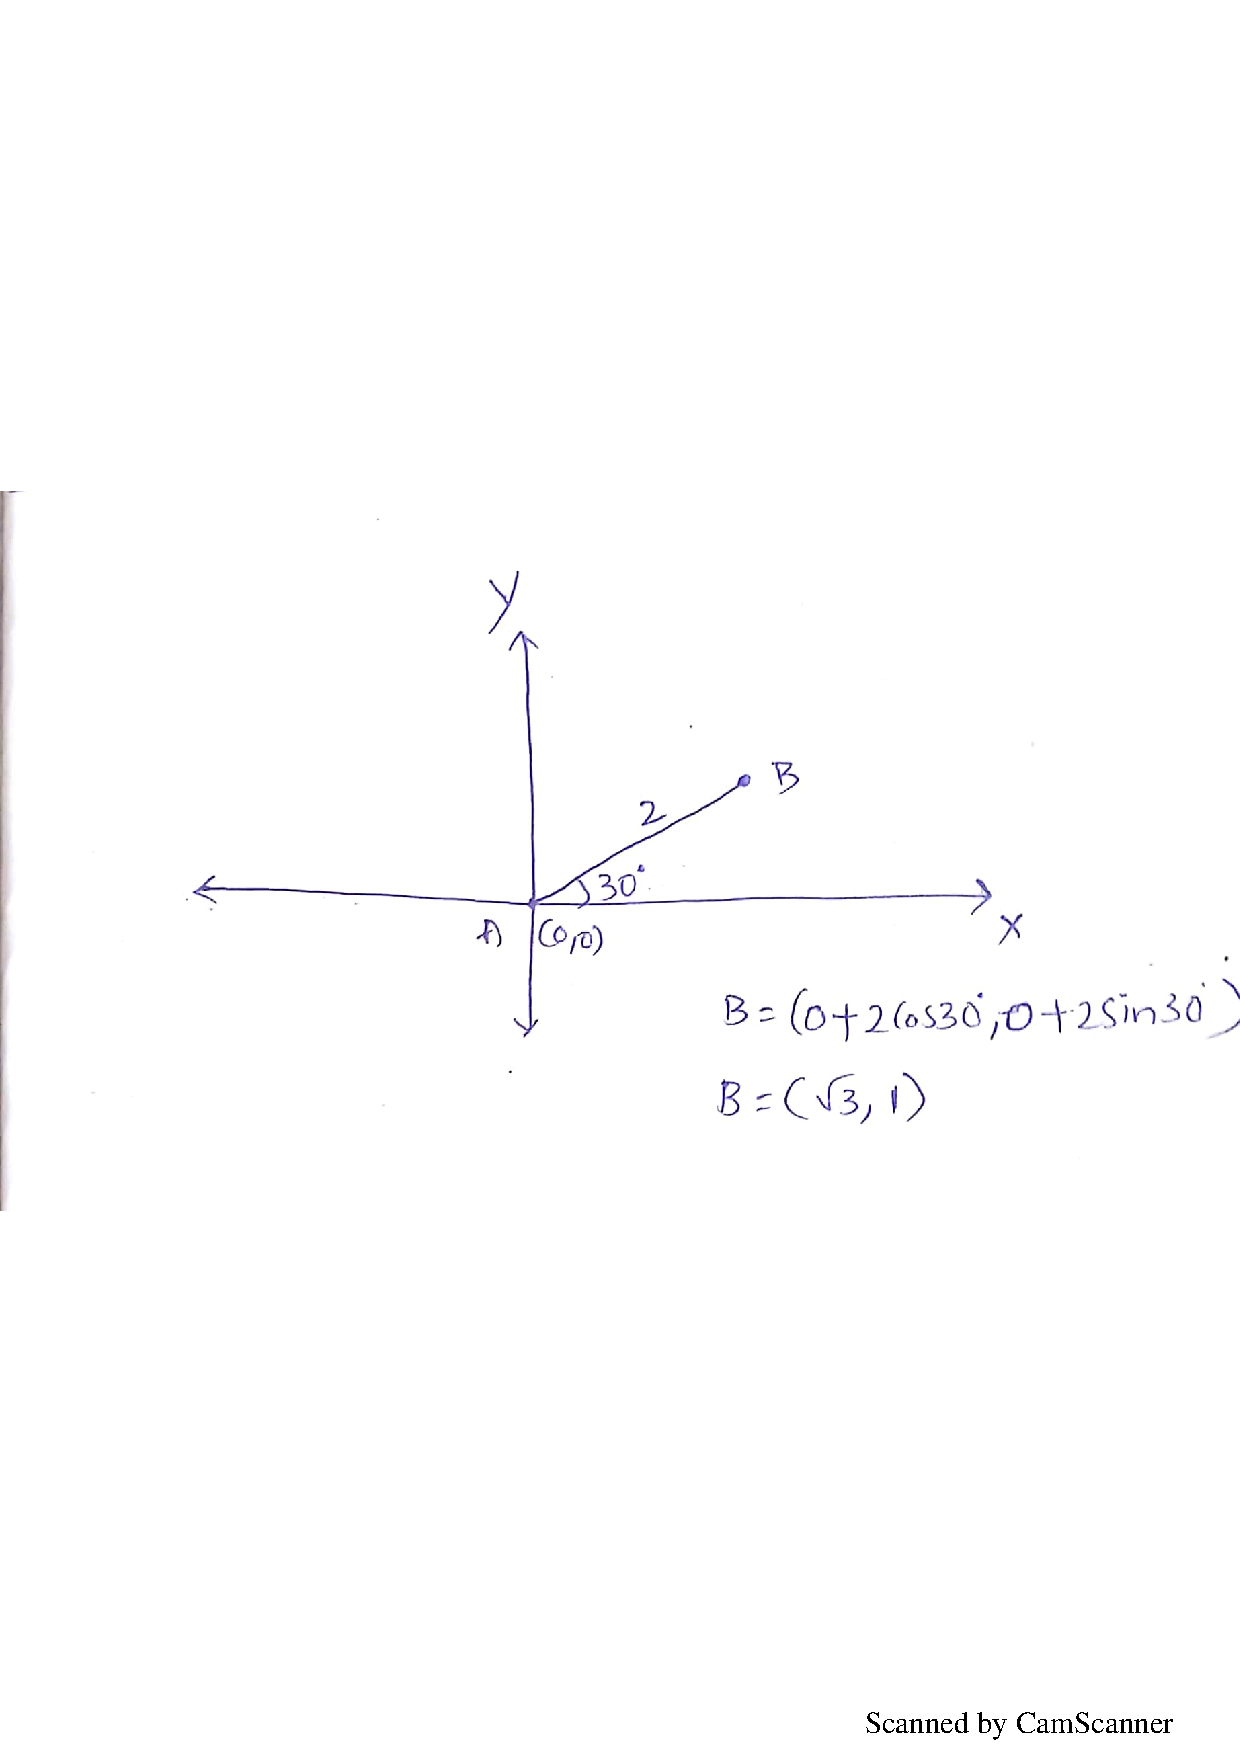
\includegraphics[scale=0.3]{pointB}
\end{figure}
\end{frame}

\begin{frame}
coordinates of the point which is 2 units away from origin and lie above x-axis (i.e Point B) can be written as

$
 B=
\begin{bmatrix}
x_{2}\\
y_{2}
\end{bmatrix}
$

$
\begin{bmatrix}
x_{2}\\
y_{2}
\end{bmatrix}=
$
$
\begin{bmatrix}
x_{1} & cos30$^\circ$ \\
y_{1} & sin30$^\circ$
\end{bmatrix}
$
$
\begin{bmatrix}
1\\
2
\end{bmatrix}
$

$
\begin{bmatrix}
x_{2}\\
y_{2}
\end{bmatrix}=
$
$
\begin{bmatrix}
0 &  \sqrt{3}/2\\
0 & 1/2
\end{bmatrix}
$
$
\begin{bmatrix}
1\\
2
\end{bmatrix}
$

$
 B=
\begin{bmatrix}
\sqrt{3}\\
1
\end{bmatrix}
$
\end{frame}

\begin{frame}

Similarly line BC makes an angle of 120$^\circ$(i.e(30+90)) with the positive direction of x-axis in anticlockwise direction
\begin{figure}[t]
\centering
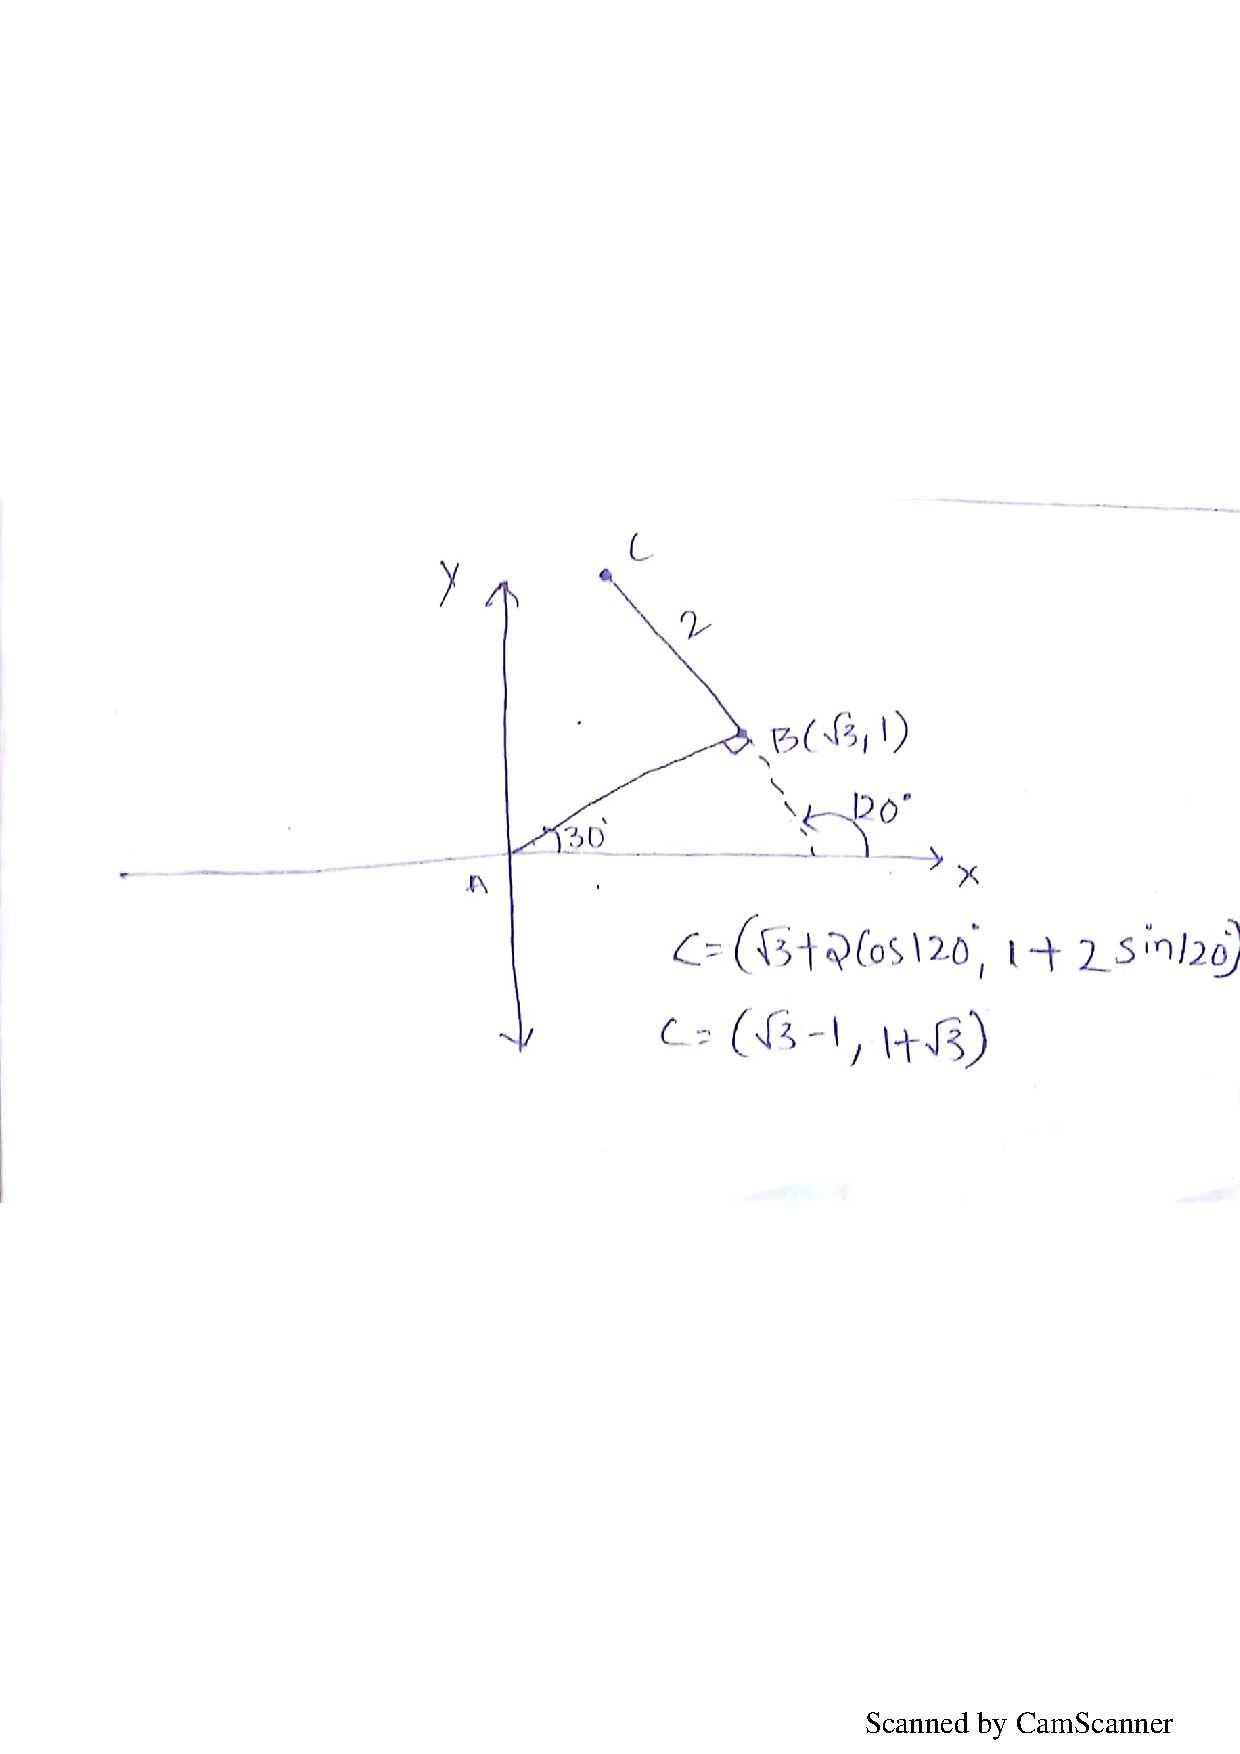
\includegraphics[scale=0.4]{pointC}
\end{figure}
\end{frame}

\begin{frame}
coordinates of the point which is 2 units away from B and lie above x-axis (i.e Point C) can be written as


$
 C=
\begin{bmatrix}
x_{3}\\
y_{3}
\end{bmatrix}
$

$
\begin{bmatrix}
x_{3}\\
y_{3}
\end{bmatrix}=
$
$
\begin{bmatrix}
x_{2} & cos120$^\circ$ \\
y_{2} & sin120$^\circ$
\end{bmatrix}
$
$
\begin{bmatrix}
1\\
2
\end{bmatrix}
$

$
\begin{bmatrix}
x_{3}\\
y_{3}
\end{bmatrix}=
$
$
\begin{bmatrix}
\sqrt{3} &  -1/2\\
1 &  \sqrt{3}/2
\end{bmatrix}
$
$
\begin{bmatrix}
1\\
2
\end{bmatrix}
$

$
 C=
\begin{bmatrix}
\sqrt{3}-1\\
1+\sqrt{3}
\end{bmatrix}
$


\end{frame}

\begin{frame}
line CD makes an angle of 210$^\circ$(i.e(120+90)) with the positive direction of x-axis in anticlockwise direction

\begin{figure}[h]
\centering
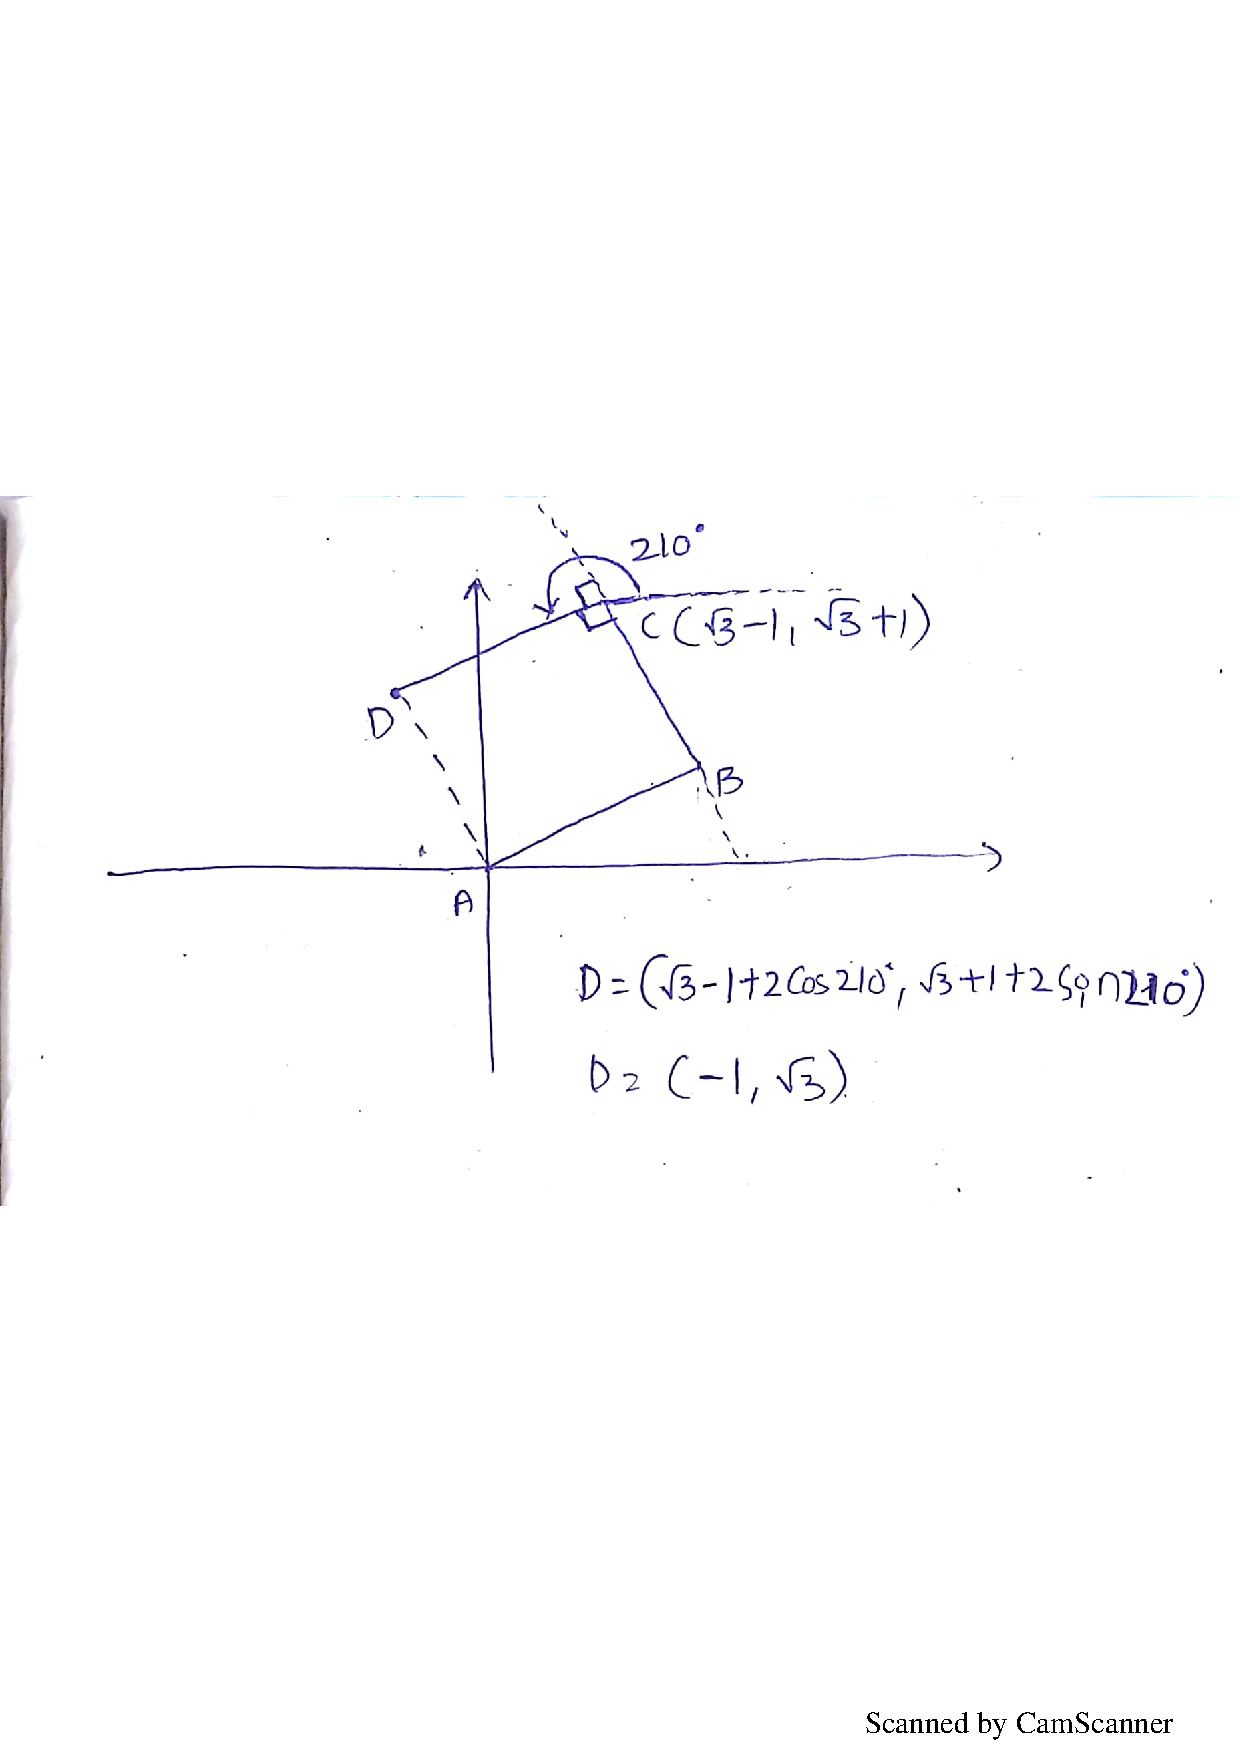
\includegraphics[scale=0.3]{pointD}
\end{figure}
\end{frame}

\begin{frame}
coordinates of the point(i.e Point D) which is 2 units away from C and also 2 units away from A (because it is a square) can be written as

$
 D=
\begin{bmatrix}
x_{4}\\
y_{4}
\end{bmatrix}
$

$
\begin{bmatrix}
x_{4}\\
y_{4}
\end{bmatrix}=
$
$
\begin{bmatrix}
x_{3} & cos210$^\circ$ \\
y_{3} & sin210$^\circ$
\end{bmatrix}
$
$
\begin{bmatrix}
1\\
2
\end{bmatrix}
$

$
\begin{bmatrix}
x_{4}\\
y_{4}
\end{bmatrix}=
$
$
\begin{bmatrix}
\sqrt{3}-1 & -\sqrt{3}/2 \\
\sqrt{3}+1 &  -1/2
\end{bmatrix}
$
$
\begin{bmatrix}
1\\
2
\end{bmatrix}
$

$
 D=
\begin{bmatrix}
-1\\
\sqrt{3}
\end{bmatrix}
$
\end{frame}

\begin{frame}
Let X be sum of x-cordinates

X=x_{1}+x_{2}+x_{3}+x_{4}

X=0+ \sqrt{3}+ (\sqrt{3}-1) + (-1)

X=1.464
\end{frame}
\end{document}




